\chapter{ギャップ増幅補題} \label{chap:gap-amplification}

DinurによるPCP定理の証明は, 与えられた制約グラフの不満足値を段階的に増幅していくアプローチに基づく.
その中核を担うのがこのギャップ増幅補題であり, 制約グラフの不満足値を増幅できることを保証する補題である.
本チャプターはこの補題の証明を与える.

\section{主張}
ギャップ増幅補題は以下のように述べられる.

\begin{lemma}{ギャップ増幅補題}{gap-amplification-lemma}
  二つの定数$c>0,\alpha\in (0,1)$, アルファベット$\Sigma$, および以下の性質を満たす決定的多項式時間アルゴリズム$A$が存在する: 
  アルゴリズム$A$は制約グラフ$G=\ip{(V,E),\Sigma,\calC}$を入力として受け取り, 次の性質を満たす別の制約グラフ$G'=\ip{(V',E'),\Sigma,\calC'}$を出力する:
  \begin{itemize}
    \item $\size(G')\le c\cdot \size(G)$.
    \item $\UNSAT(G)=0$ならば$\UNSAT(G')=0$.
    \item $\UNSAT(G)>0$ならば$\UNSAT(G')\ge \min\{\alpha, 2\cdot \UNSAT(G)\}$.
  \end{itemize}
\end{lemma}

PCP定理(\cref{thm:PCP-CSP-theorem})の証明は, この補題を繰り返し適用することによって得られる.

\begin{proof}[\cref{lem:gap-amplification-lemma}の下での\cref{thm:PCP-CSP-theorem}の証明.]
  3彩色問題のインスタンスを入力として受け取り, その制約グラフを$G_0$とし, 頂点数を$n$とする.
  この制約グラフは単純グラフであるため, $\UNSAT(G_0)=0$もしくは$\UNSAT(G_0)\ge \frac{1}{n^2}$である.
  \cref{lem:gap-amplification-lemma}のアルゴリズムを$A$とし, 各$i=1,\dots,\ceil{2\log_2 n}$について, 制約グラフ$G_i$を
  $G_i = A(G_{i-1})$として定義し, 最終的に得られる制約グラフを$G'=G_{\ceil{2\log_2 n}}$とする.
  各$G_i$のサイズは$\size(G_i) \le c\cdot \size(G_{i-1})$であるため, $\size(G')\le c^{\ceil{2\log_2 n}}\cdot \size(G_0)=\size(G_0)^{O(1)}$である.
  従って$G'$は多項式時間で構成できる.

  また, 不満足値については, 以下のようになる:
  \begin{itemize}
  \item もしも$G_0$がYesインスタンスであるならば, 全ての$i$に対して$G_i$もYesインスタンスであり, 特に$\UNSAT(G')=0$である.
  \item もしも$G_0$がNoインスタンスであるならば, $\UNSAT(G_0)\ge \frac{1}{n^2}$かつ$\UNSAT(G_i)\ge \min\{\alpha, 2\cdot \UNSAT(G_0)\}$であるため, $\UNSAT(G')\ge \min\qty{\alpha, 2^{2\log_2 n}\cdot \frac{1}{n^2}}=\alpha$である.
  \end{itemize}
\end{proof}

ギャップ増幅補題では与えられた制約グラフを変換していく.
表記の簡略化のため, グラフに対する性質を表す用語を制約グラフにもそのまま適用することとする.
例えば$(V,E)$が連結であるときに$G=\ip{(V,E),\Sigma,\calC}$は連結であるという.
また, $(V,E)$が正則であるときに$G=\ip{(V,E),\Sigma,\calC}$は正則であるという.


\section{制約グラフの定数次数エクスパンダー化}

まず, 与えられた制約グラフを, 不満足値をそれほど減らさずに定数次数の正則性かつエクスパンダー性を持つように変形する.

\begin{lemma}{定数次数エクスパンダー化}{constant-degree-expanderization-lemma}
  ある定数$\lambda<1$, $d\in\Nat$, $c>0$, $\beta>0$が存在して,
  任意の制約グラフ$G=\ip{(V,E),\Sigma,\calC}$を入力として受け取り, 以下の性質を満たす別の制約グラフ$G'=\ip{(V',E'),\Sigma,\calC'}$を出力する決定的多項式時間アルゴリズム $A$ が存在する:
  \begin{itemize}
    \item $G'$は自己ループを持つ$d$-正則$\lambda$-エクスパンダーである.
    \item $\size(G') \le c\cdot \size(G)$.
    \item $\UNSAT(G)=0$ならば$\UNSAT(G')=0$.
    \item $\UNSAT(G') \ge \beta\cdot\UNSAT(G)$.
  \end{itemize}
\end{lemma}

この補題の証明は次数の削減とエクスパンダー化の二つのステップからなる.

\subsection{次数の削減}

まず, 与えられた制約グラフを定数次数の正則グラフに変換する補題を示す.
この変換によって$\UNSAT$の値は定数倍しか変化しない.

\begin{lemma}{次数削減補題}{degree-reduction-lemma}
  ある定数$d\in\Nat$, $c>0$が存在して, 任意の制約グラフ$G=\ip{(V,E),\Sigma,\calC}$を入力として受け取り, 以下の性質を満たす別の制約グラフ$G'=\ip{(V',E'),\Sigma,\calC'}$を出力する決定的多項式時間アルゴリズム $A_1$ が存在する:
  \begin{itemize}
    \item $G'$は$d$-正則である.
    \item $\abs{V'} \le 2\abs{E}$.
    \item $\UNSAT(G)=0$ならば$\UNSAT(G')=0$.
    \item $\UNSAT(G') \ge c\cdot \UNSAT(G)$.
  \end{itemize}
\end{lemma}

\begin{proof}

与えられた制約グラフを$G=\ip{(V,E),\Sigma,\calC}$とし, 変換によって得られる制約グラフを$G'=\ip{(V',E'),\Sigma,\calC'}$とする.
フォーマルな構成を与える前に, まず図例を先に示す.

\begin{figure}[h]
  \centering
  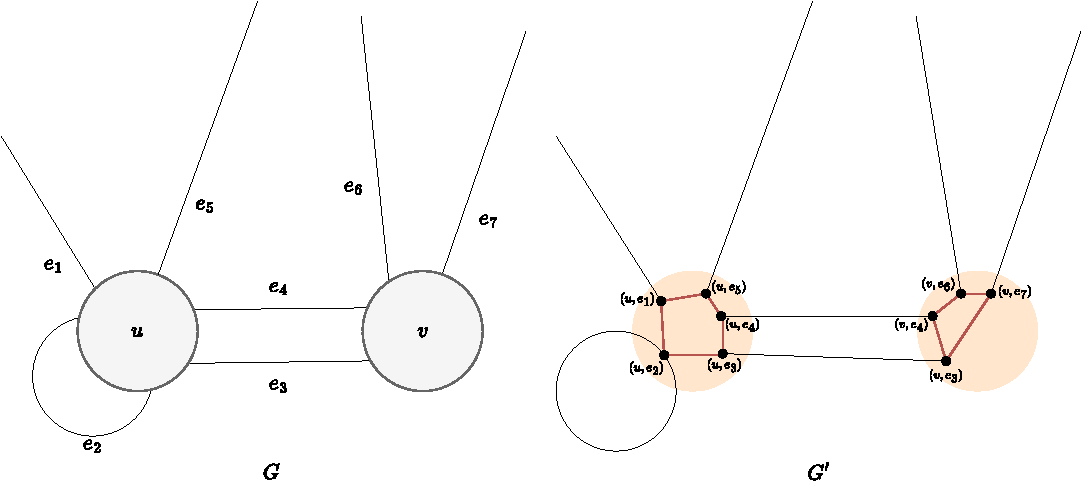
\includegraphics[width=\textwidth]{images/degree_reduction.pdf}
  \caption{次数削減変換の例. 橙色の内部の頂点集合がクラウドであり, クラウド内の辺は\cref{thm:construction-of-expander-graph}によって構成されるが, ここでは図の簡単のため$X_d$を長さ$d$の閉路としている. この例の場合, $G'$は$3$-正則となる.}
  \label{fig:degree-reduction}
\end{figure}

元のグラフの各頂点$u\in V$に対し, 
\[[u]=\qty{ (u,e) \in \{u\}\times E \colon e=\{u,v\} \text{ for some } v\in V }\]
を(この証明のローカルな用語として)\emph{$u$-クラウド}と呼ぶことにする.
新しい頂点集合$V'$は$V'=\bigcup_{u\in V} [u]$である.
すなわち, $u$をそれに接続する辺の本数(自己ループは1個分としてカウント)だけコピーして得られる集合が$[u]$である.

次に辺集合$E'$を以下のように構成する.
まず, $(X_n)_{n\in\Nat}$を\cref{thm:construction-of-expander-graph}によって構成される$n$頂点$d_0$-正則$\lambda$-エクスパンダーの族とする.
元のグラフの各頂点$u\in V$に対し, $d=\abs{[u]}$としたとき, 頂点集合$[u]$上で$X_d$と同型なグラフを構成し, それを$([u],E_u)$とする.
このとき, 各$u$-クラウド内部の辺集合$E_{\mathrm{inner}}$は
\begin{align*}
  E_{\mathrm{inner}} = \bigcup_{u\in V} E_u
\end{align*}
とする.
次に異なるクラウド間を繋ぐ辺集合$E_{\mathrm{outer}}$を
\begin{align*}
  E_{\mathrm{outer}} = \qty{\qty{ (u,e), (v,e) } \colon e\notin [u]\cap[v]}
\end{align*}
とする.
このとき, グラフ$G'$の辺集合$E'$は
\begin{align*}
  E' = E_{\mathrm{inner}} \cup E_{\mathrm{outer}}
\end{align*}
となる.

次に各辺$e'\in E'$の制約$c'_{e'}$を以下のように定める:
\begin{itemize}
\item 辺$e'\in E_{\mathrm{outer}}$がクラウド間をつなぐ辺ならば, その制約は対応する元の辺$e$の制約と同じとする.
すなわち, $e'=\qty{ (u,e), (v,e) }$ならば, $c'_{e'}=c_e$である.
\item 辺$e'\in E_{\mathrm{inner}}$がクラウド内部の辺ならば, その制約は全集合, すなわち$c'_{e'}=\Sigma^2$とする.
\end{itemize}

このようにして得られる制約グラフ$G'=\ip{(V',E'),\Sigma,\calC'}$が補題の主張を全て満たすことを確認する.
まず, $G'$は$(d_0+1)$-正則である.
実際, $G'$の各頂点$(u,e)\in V'$に接続する辺は, クラウド内の辺が$d_0$本, クラウド間の辺が$1$本である.
また, $V'$の要素数は次数の総和に等しいため, $\abs{V'}\le 2\abs{E}$を満たす ($2\abs{E}-\abs{V'}$は元のグラフの自己ループの個数分に等しい).
次に, $\UNSAT(G)=0$ならば$\UNSAT(G')=0$である.
実際, 元の制約グラフの全ての制約を満たす割り当て$a\colon V\to\Sigma$に対し, $G'$の割り当て$a'\colon V'\to\Sigma$を
\begin{align*}
  a'(u,e) = a(u)
\end{align*}
と定めると, $a'$は$G'$の制約を満たす (クラウド内の辺に対応する制約は全て満たされ, クラウド間の辺に対応する制約は$a$の取り方により全て満たされることがわかる).

最後の主張, すなわち$\UNSAT(G') \ge c\cdot \UNSAT(G)$を背理法で示すために, これが成り立たないと仮定する.
このとき, ある$G'$の割り当て$a'\colon V'\to\Sigma$が存在して$\UNSAT_{G'}(a')<c\cdot \UNSAT_G(a')$となる.
この割り当て$a'$に対し, 元のグラフ$G$の割り当て$a\colon V\to\Sigma$を
\begin{align*}
  a(u) = \Maj((a'(u,e))_{(u,e) \in [u]})
\end{align*}
と定める. ここで$\Maj(\cdot)$は多数決関数であり,
タイは任意に選ぶとする.
例えば$\Maj(1,2,2)=2$, $\Maj(1,2,3,3)=3$, $\Maj(1,2,2,3,3)=2$である ($\Maj(1,2,2,3,3)=3$としても良いが, ここでは便宜上小さい方の数字を採用している).
以下, このようにして定まる新たな割り当て$a\colon V \to \Sigma$が
$\UNSAT_G(a) < \UNSAT(G')$となることを示すことによって矛盾を導く (この不等式は$\UNSAT(G)$の定義に反している).

以降, 割り当て$a'\colon V'\to\Sigma$に対し, 頂点$(u,e)\in V'$への割り当て$a'(u,e)$を頂点$(u,e)$の\emph{意見}と呼ぶこととする.
同様に, 割り当て$a\colon V\to\Sigma$に対し, 頂点$u\in V$への割り当て$a(u)$を頂点$u$の意見と呼ぶこととする.
直感的には頂点$u$の意見は対応する$u$-クラウド内の頂点の意見の多数決である.


辺集合$F\subseteq E$を割り当て$a$によって充足されない辺の集合, すなわち
\begin{align*}
  F = \qty{ e=\{u,v\}\in E \colon u<v\text{ and } (a(u),a(v)) \not\in c_e}
\end{align*}
と定義する.
ここで$\calC = (c_e)_{e\in E}$は元の制約グラフ$G$の制約である.
同様に, $F'\subseteq E'$を割り当て$a'$によって充足されない辺の集合とする.
このとき$\UNSAT_G(a) = \frac{|F|}{|E|}$および$\UNSAT_{G'}(a') = \frac{|F'|}{|E'|}$である.
頂点部分集合$S\subseteq V'$を$a$の多数決で選ばれなかった意見を持つ頂点の集合, すなわち
\begin{align*}
  S = \qty{ (u,e) \in V' \colon a(u) \ne a'(u,e)}
\end{align*}
と定義し, 各$v\in V$に対し$S^v = S\cap [v]$とし, 各$\sigma\in \Sigma$に対し$S^v_\sigma = \qty{ (u,e)\in S^v \colon a'(u,e)=\sigma }$とする (\cref{fig:majority-degree-reduction}).
なお, $\sigma\in\Sigma$が多数決の意見 (すなわち$\sigma=a(v)$)のとき, $S^v_\sigma=\emptyset$とする.

\begin{figure}[h]
  \centering
  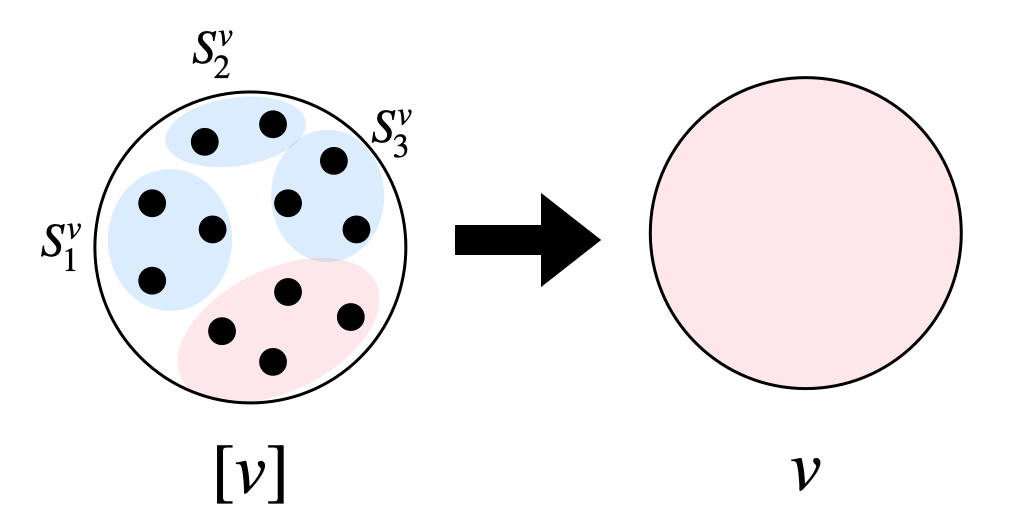
\includegraphics[width=\textwidth]{images/majority_degree_reduction.png}
  \caption{多数決によって選ばれなかった$v$-クラウド内の頂点の集合を$S_v\subseteq [v]$とする. \label{fig:majority-degree-reduction}}
\end{figure}

以下の二つのケースを考える:

\paragraph*{ケース1. $\abs{S} \ge \frac{\UNSAT_G(a)}{2}\abs{E}$の場合.}

各頂点$v\in V$に対し, 

\paragraph*{ケース2. $\abs{S} < \frac{\UNSAT_G(a)}{2}\abs{E}$の場合.}













\end{proof}

\subsection{エクスパンダー化}


\section{制約グラフのべき乗}

\section{アルファベット削減}



